\documentclass[14pt]{article}
\usepackage{url}
\usepackage{hyperref}
\usepackage{amsmath}
\usepackage{mathtools}
\usepackage{extsizes}
\usepackage{titling}
\usepackage{siunitx}
\usepackage{graphicx}
\usepackage[shortlabels]{enumitem}
\usepackage[margin=0.75in]{geometry}
\usepackage{indentfirst}
\usepackage{caption}

\newcommand{\bd}{\textbf}
\newcommand{\ul}{\underline}

\setlength{\droptitle}{-5em} 

\title{Exam 1}
\author{Mitchell Meier}
\date{\today}

\begin{document}

\maketitle

\section*{Problem 1}
\subsection*{Introduction}
For this report, we are going to analyze a set of data describing the past data scores for a class, with some information about each student included for context. Including these variables about the student, in addition to their exam scores, will hopefully help us in determing if there is an coorelation between a student's exam scores and their other traits \\

\noindent For the columns in our data set, we have:

\begin{itemize}
\item \emph{Section}, which is a categorical nominal data type that lists the section number the student was in (either Section 101 or Section 102)
\item The next three columns, \emph{Exam 1, 2, and 3}, are all quanitive discrete data types. These columns are the primary focus of our data set
\item After the exam scores we have the \emph{Attendance} column, which is a categorical ordinal data type with four possible values (listed highest to lowest): frequently, occasionally, rarely, never
\item The next column, \emph{College level}, is also a categorical ordinal data type. The values for this colum are: senior, junior, sophmore, and freshman
\item Our last column is \emph{Major}, which is a categorical nominal data type \\
\end{itemize}
\pagebreak

\noindent Our assigned objectives for this study are to find if a student's:

\begin{enumerate}
\item attendance has any impact on their exam scores
\item exam 1 score impacts their exam 2 and exam 3 scores
\item attendance is dependent on their college level
\item college level has any impact on their exam scores
\item major has any impact on their exam scores
\item section has any impact on their exam scores
\item section has any impact on their attendance 
\end{enumerate} 

Our main goal heading into our analysis is to see how our columns influence a student's exam scores. Hopefully we will be able to analyze this data to a point where we can predict how a student will score on their exams based on their other traits. We may also discover by looking at the individual exam data that the exam number may also factor into a student's success \\ 

\subsection*{Analysis}
For the analysis section, we'll be splitting up our analysis between each objective, and use graphs and statistical summaries to make inferences on the data. To help with our analysis, I decided to add one additional column to our data, called \emph{Exam Average}, which contains the average score for each student out of their three exams. I believe this column should still fall under the requirement of "provided data", since it is entirely derived from provided data. This column will make it easier in comparing exam scores to other attributes \pagebreak

\begin{enumerate}
\item

Attendance seems to have one of the most distinct relationships with average exam score. As we can see in our coorelation graph, a large majority of the highest scores were from student that attened class frequently. In fact, out of the 44 highest averaging student, 42 of them visted class frequently, and the other two visited occassionally. The average (of exam averages) for students who visited class frequently and occassionally were high as well, with only one data point in each that could be considered an outlier. I believe it is safe to say that students who attend STAT 3113 more frequently will be more likely to do better on their exams.

\vspace{5em}

\begin{figure}[h]
\caption*{Student's attendance and average Exam Score}
\centering
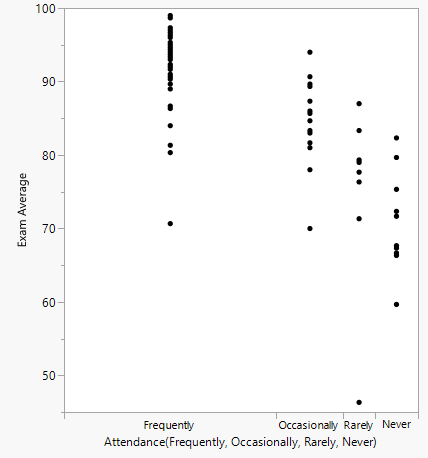
\includegraphics{exam1/1.png}
\end{figure}

\pagebreak

\item
Students in STAT 3113 seem to be consistent between tests on average. There is a steady trend showing that the score a student gets on exam one is similar to the scores they get on exam two and three. There do seem to be cases where this does not hold true, however, each exam has some outliers where a couple students have drasticly different score between exams. But for the majority of students, this trend does in fact hold true 

\begin{figure}[h]
\caption*{Student's Exam 1 score and Exam 2 score}
\centering
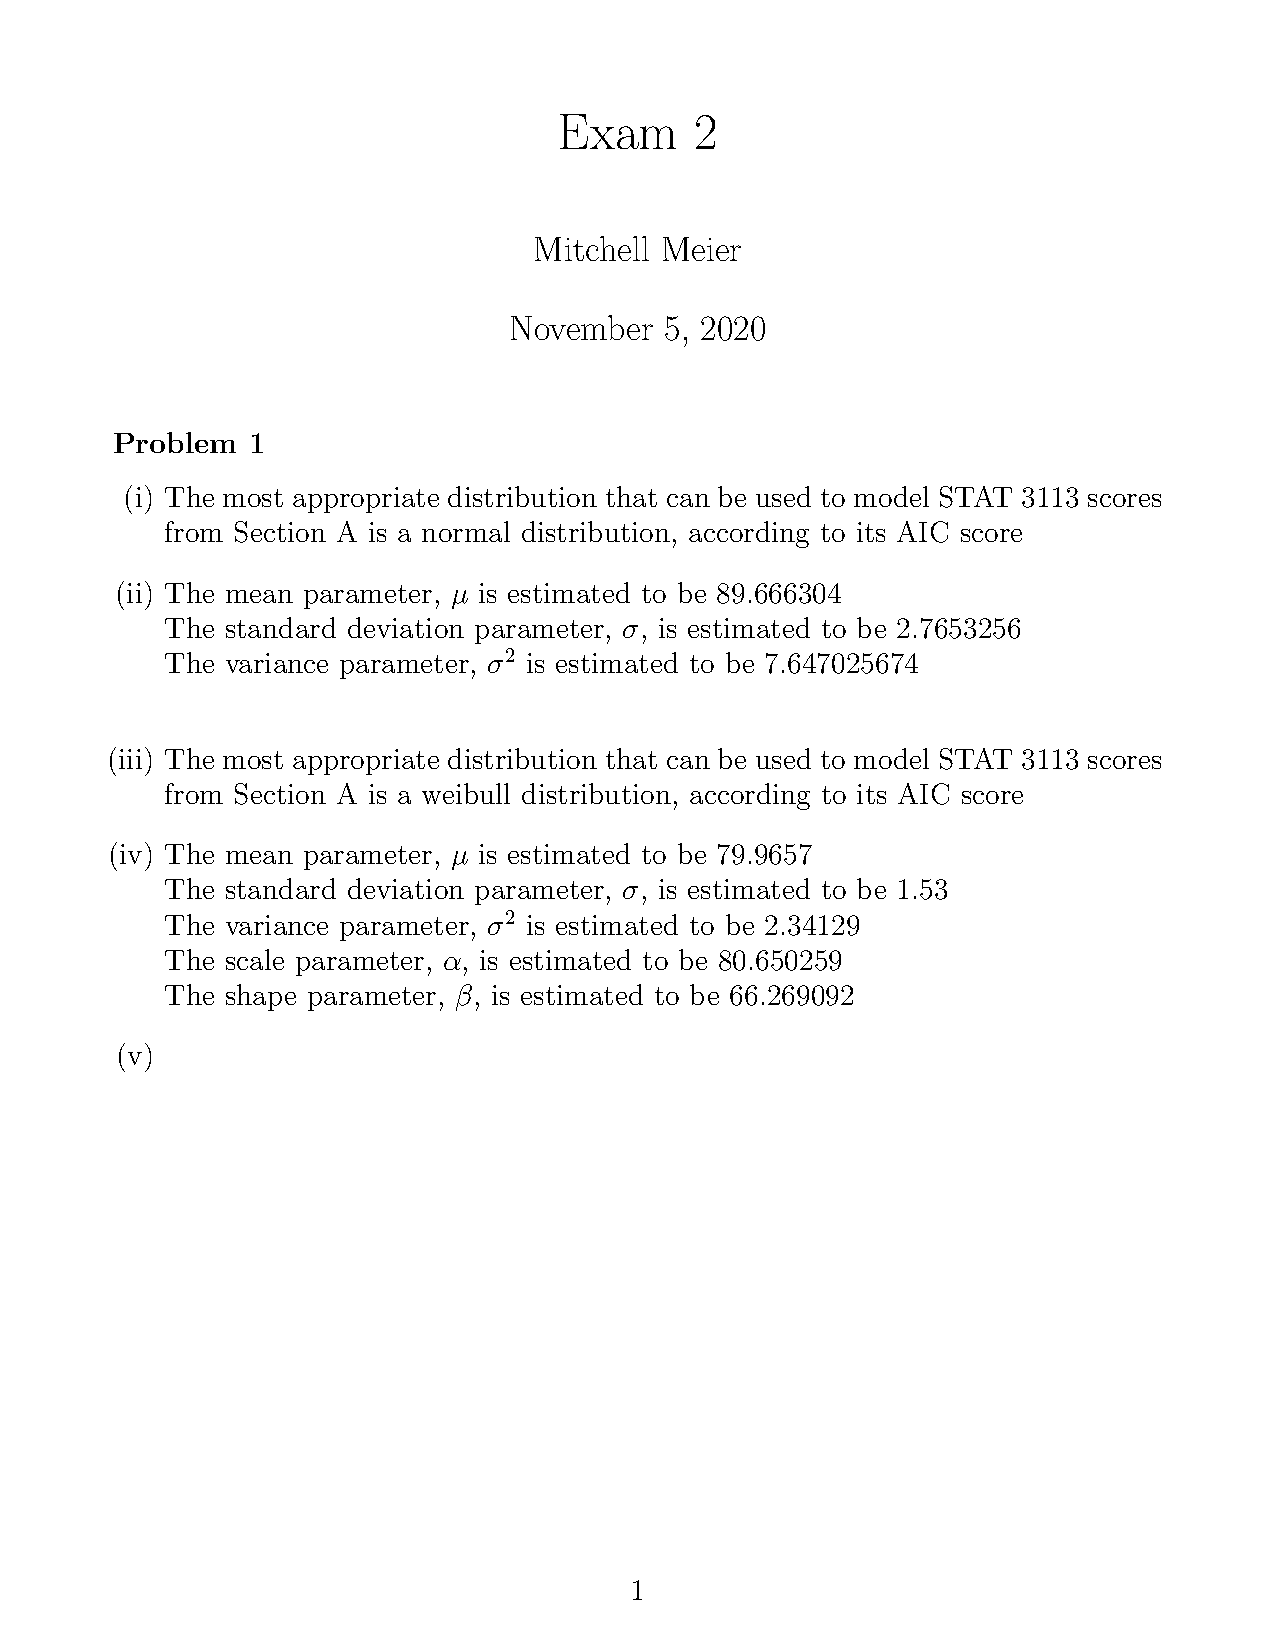
\includegraphics[scale=0.6]{exam1/exam2.png}
\end{figure}

\begin{figure}[h]
\caption*{Student's Exam 1 score and Exam 3 score}
\centering
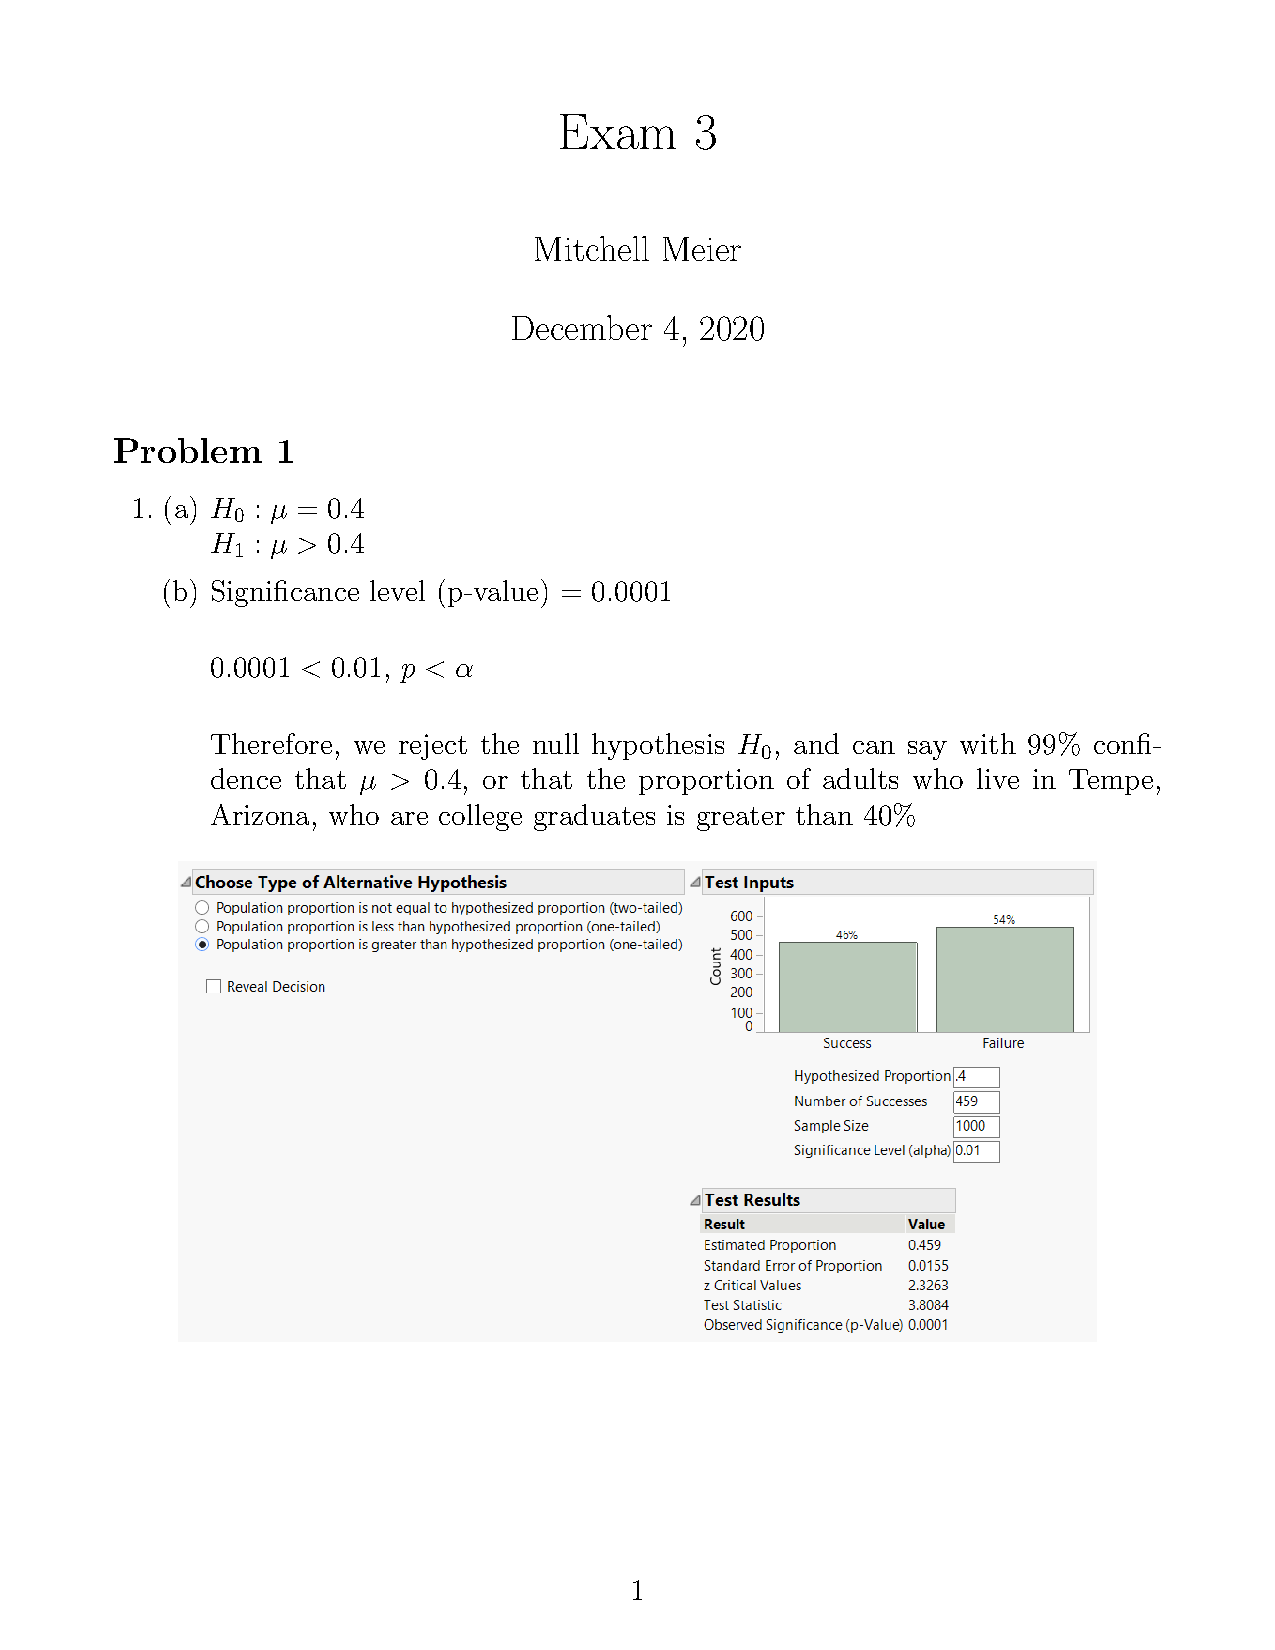
\includegraphics[scale=0.6]{exam1/exam3.png}
\end{figure}

\pagebreak

\item
Since this study had a disproportiante amount of upper class men to lower class men, I decided the best way to evaluate the coorelation between attendance and college level was a contour graph. The contour graph will give more of an emphasis on the proportion of students (per class level) that atteneded class frequently, rather than just the number. From looking at the contour graph, there seems to be negligable difference between class levels when it comes to attendance. All classes had a large chunk of their students attending frequently, with a slightly smaller percentage of students attend occasionally. Only a slightly larger percentage of sophmores and juniors attened class rarely or never compared to freshman are seniors.

\vspace{2.5em}

\begin{figure}[h]
\caption*{Student's Attendance by College Level}
\centering
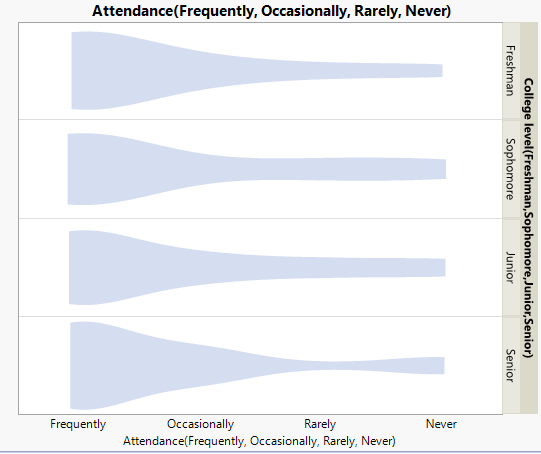
\includegraphics{exam1/3.png}
\end{figure}

\pagebreak

\item
The relationship between class level and exam scores seems to be similar to our last relationship. Our boxplots show that the interquartile ranges for each class level are very close to each other, as well as the means. The sophmore class is the only class level with a slightly lower mean compared to the other class levels, but this could simply be attributed to the sophmore class having the lowest outlier by far.

\vspace{2.5em}

\begin{figure}[h]
\caption*{Student's average Exam Score by College Level}
\centering
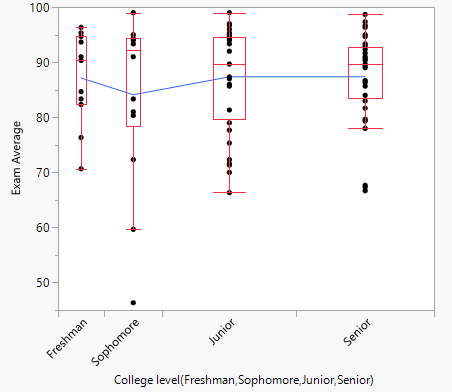
\includegraphics[scale=1.25]{exam1/4.png}
\end{figure}

\pagebreak

\item
According to our data, the top 3 performing majors, based on average exam scores, are Architectrual Engineering, Mechanical Engineering, and Mining Engineering. However, when we compare the reliability of this data to the rest of our data, it is much lower. This is because we have a wide variety of majors that have taken STAT 3113, so our data for most of these majors consists of a comparibly smaller sample size. With that being said, I believe there is insufficent data here to draw a strong conclusion on which major's have a better chance of obtaining higher exam scores.

\vspace{2em}

\begin{figure}[h]
\caption*{Student's average Exam Score by College Level}
\centering
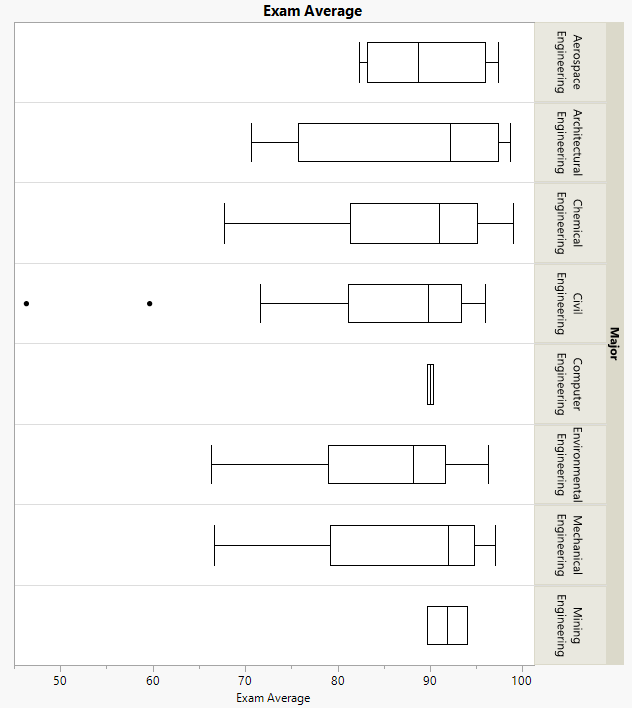
\includegraphics[scale=0.75]{exam1/5.png}
\end{figure}

\pagebreak

\item
Using a histogram to analyze our section data, it seems that there is not a big difference between taking section 101 and section 102. Both sections have similar data distributions. If we were to point out one difference, however, section 101 seems to be slightly more left skewed, though it is barely noticeable. Odds are that section number will not have an impact on a  student's exam score.

\vspace{2em}

\begin{figure}[h]
\caption*{Student's average Exam Score by College Level}
\centering
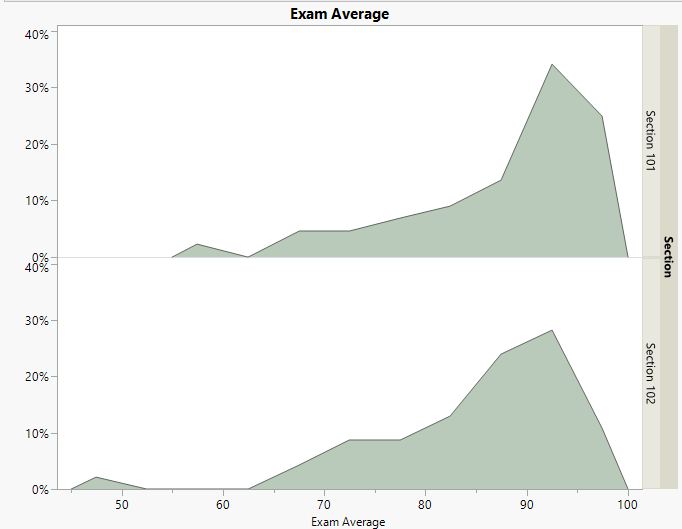
\includegraphics{exam1/6.png}
\end{figure}

\pagebreak

\item \textbf{Additional Objective:}
For my additional objective, I wanted to see if students' attendance was coorelated to section number at all. If it was, there could be a good amount of factors not listed in our data that, if listed, could provide a good deal more insight into why student's grades are high or low. Perhaps a certain section is too early in the morning for students to attend, or they don't attend because they find their paticular section's lectures uninteresting (very unlikely for our class :) ). Looking at our data, it seems that there is a slight different between the attendance in our two sections. Less students are attending frequently in section 102 than 101, though not by a wide margin (less than 10 percent). 

\vspace{5em}

\begin{figure}[h]
\caption*{Student's Attendace by Section Number}
\centering
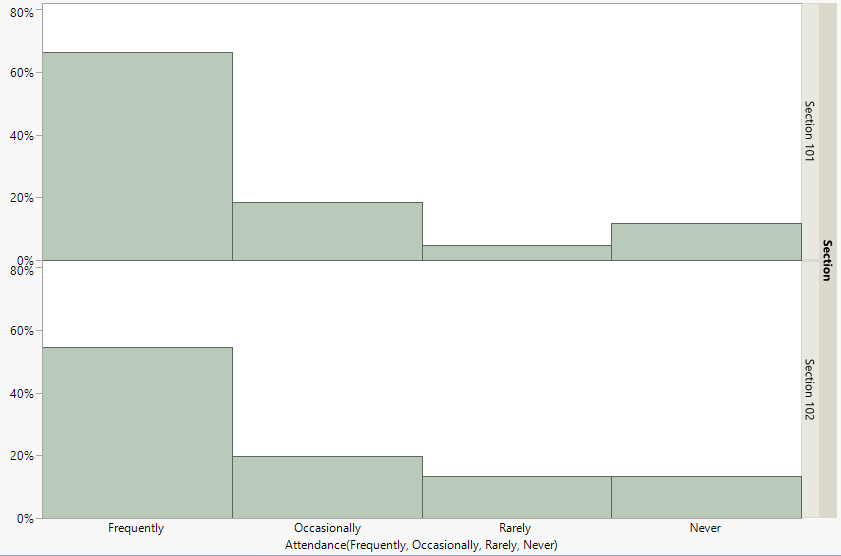
\includegraphics[scale=0.75]{exam1/7.png}
\end{figure}

\pagebreak

\end{enumerate}


\subsection*{Conclusion}
To summarize the conclusion's by objective: 

\begin{enumerate}
\item Attendace heavily impacts exam scores. The data infers that students who attended class more often are more likely to score higher on exams
\item Students who were the higher scores on exam one tended to also be higher scores on exams 2 and 3. The data did not guarantee that students would keep their high scores, but in the majority of cases they would.
\item The data suggested that students attended class slightly more than juniors and sophmores, but not by a wide margin. The most likely assumption to be true here is that a student's college level will have little impact on their attendance
\item Similar to how college year coorelated with attendance, it also does not seem to influence exam score that much. The best reccomendation to make to a student regarding when to take STAT 3113 is to not worry about what year is generally best to take it. It is more likely to be dependent on the student's course load by year 
\item Major may or may not impact exam score. Going off the data in our study alone, a case could be made for certain major's excelling more in this class. However, not only was there not too much difference between majors, but the sample size for each major is quite low for this experiment. So to conclude on this objective, I believe it can be hypothesised that major does not impact exam score, but I am not confident enough with our sample size to say that with certainty
\item The data shows that the students from section 101 and 102 have similar exam scores. So going off this realtionship alone, it would be easy to conclude that no one section has an inherent advantage. However, more factors are usually involved when it comes to differences between sections, so I decided to explore section relations more with my additional objective
\item In our addditional objective, the data shows that there is a slight coorelation between attendance and section number. Students in section 101 seem more inclined to attend class for whatever reason compared to 102. This could be due to a variety of different factors within the section, or it could just be due to the kinds of students in each section. More coorelation analysist, and possibly even new data points, would be needed to find the reason for this difference in attendance
\end{enumerate}

\section*{Problem 2}

\end{document}